\documentclass{scrartcl}
\usepackage{polski}
\usepackage[utf8]{inputenc}

\usepackage{hhline}
\usepackage{enumerate}
\usepackage{graphicx}
\usepackage{epstopdf}
\usepackage{float}
\usepackage{amsmath}
\usepackage{geometry} 
\usepackage{multirow}
\usepackage{mathtools}
\usepackage{paralist}
\usepackage{listings}
\usepackage{xpatch}


\newgeometry{tmargin=2.5cm, bmargin=2.5cm, lmargin=2.4cm, rmargin=2.4cm} 

\title{Metody planowania i analizy eksperymentów\\Zadanie domowe 2}
\subtitle{Zastosowanie metod wnioskowania statystycznego na przykładzie zbioru danych \textit{Abalone}}

\author{\textbf{Prowadzący:} dr inż. Adam Zagdański \\ 
        \textbf{Student:} Piotr Bielak, 218 137\\WT TN 9:15}

\date{Wrocław, 31 maja 2018r.}

\begin{document}
\maketitle
\pagebreak
\section{Wprowadzenie}
Do realizacji zadania domowego użyto zbiór danych \textbf{Abalone}, który został
zaczerpnięty z repozytorium danych \textit{UCI Machine Learning Repository}. 
Zbiór ten zawiera dane opisujące ślimaki morskie i został przygotowany w celu 
predykcji ich wieku. W celu przeprowadzenia estymacji (punktowej i przedziałowej)
oraz testu statystycznego został wykorzystany język R w oparciu
o wbudowane pakiety tego języka (brak dodatkowych zewnętrznych pakietów).

\section{Wyniki}

\subsection{Estymacja punktowa}
W przypadku estymacji punktowej celem jest wyznaczenie pojedynczej liczby 
opisującej dany parametr rozkładu wybranej zmiennej losowej. W poniższym przykładzie
została wybrana cecha opisująca liczbę pierścieni (która jest równoważna z wiekiem
osobnika). Używając kolejne wartości liczby pierścieni uzyskane w trakcie eksperymentu
obliczono średnią oraz wariancję próbkową. Wzory zostały podane poniżej:
$$ Mean(x) = \frac{1}{n} \sum_{i = 1}^{n}x_i; $$
$$ Var(x) = \frac{1}{n - 1}\sum_{i = 1}^{n}(x_i - Mean(x))^2$$
Z obliczeń uzyskano następujące wartości:
\begin{itemize}
  \item{średnia próbkowa: 9.93,}
  \item{wariancja próbkowa: 10.40.}
\end{itemize}
Poniższy obrazek przedstawia rozkład wartości atrybutu \textit{Rings} (l. pierścieni) wraz
z dopasowanym rozkładem normalnym z parametrami wyznaczonymi powyżej.

\begin{figure}[H]
  \center
  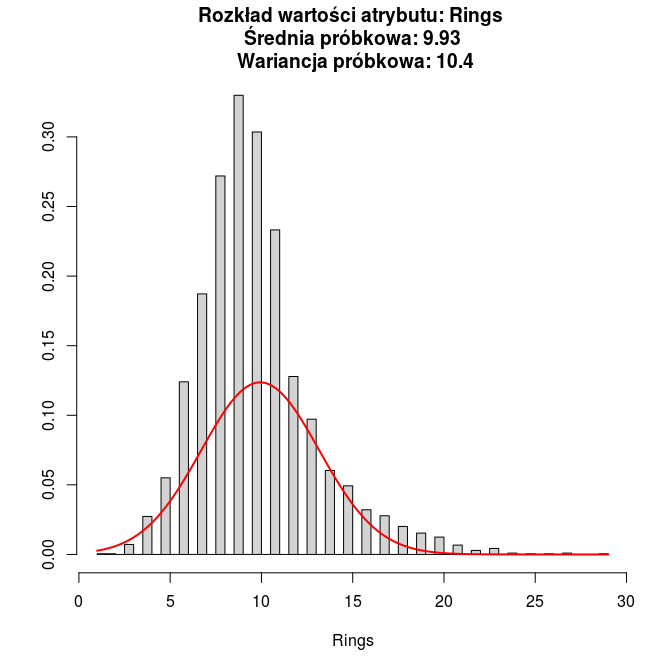
\includegraphics[width=0.6\textwidth]{imgs/rings_estimated.png}
  \caption{Wyniki estymacji punktowej dla atrybutu "Rings".}
\end{figure}

\subsection{Estymacja przedziałowa}
W celu przeprowadzenia estymacji przedziałowej zostały zaimplementowane funkcje
do obliczania granic przedziałów:
\begin{itemize}
  \item{estymacja średniej w oparciu o \textbf{rozkład normalny} (n >> 30),}
  \item{estymacja wariancji w oparciu o \textbf{rozkład chi-kwadra}.}
\end{itemize}
Poniższa tabela przedstawia wyniki estymacji dla atrybutu \textit{Rings} dla różnych
wartości poziomu ufności.

\begin{table}[H]
  \center
  \begin{tabular}{c|ccc}
    \textbf{Poziom ufności} & \textbf{Parametr} & \textbf{L} & \textbf{R} \\ \hline
    \multirow{2}{*}{0.01}  & średnia            &  9.932     & 9.936 \\
                           & wariancja          &  10.397    & 10.402 \\ \hline

    \multirow{2}{*}{0.05}  & średnia            &  9.924     & 9.944 \\
                           & wariancja          &  10.385    & 10.414 \\ \hline

    \multirow{2}{*}{0.10}  & średnia            &  9.913     & 9.954 \\
                           & wariancja          &  10.371    & 10.428 \\ \hline
                           
    \multirow{2}{*}{0.50}  & średnia            &  9.825     & 10.042 \\
                           & wariancja          &  10.247    & 10.554 \\ 
                           
  \end{tabular}

  \caption{Wyniki estymacji przedziałowej.}
\end{table}

\begin{figure}[H]
  \center
  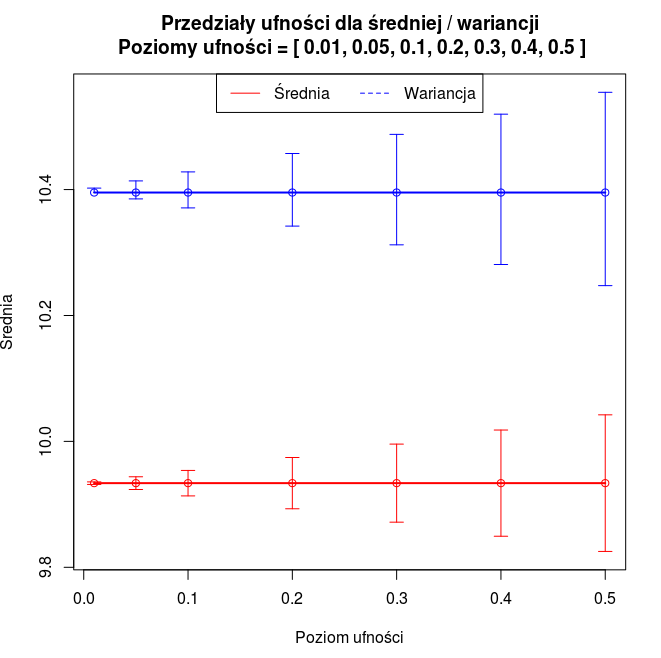
\includegraphics[width=0.5\textwidth]{imgs/int_estim.png}
  \caption{Przedziały ufności dla różnych poziomów ufności.}
\end{figure}
Można zauważyć, że dla mniejszych poziomów ufności (większych wartości
parametru \textit{alpha}) przedział ufności jest węższy i zaczyna skupiać
się wokół, odpowiednio, średniej oraz wariancji próbkowej.

\pagebreak

\subsection{Weryfikacja hipotezy statystycznej}
W ramach badania testu statystycznego (weryfikacji hipotezy statystycznej) wykorzystano
funkcję \textbf{t.test(...)} z pakietu R. Pozwala ona na wykonanie testu t-Studenta dla
dwóch prób niezależnych. Test przeprowadzono dla atrybutu \textbf{Rings} dla osobników
męskich oraz żeńskich (2 próby). Przyjęto różne poziomy istotności oraz różne hipotezy
alternatywne. Wyniki zostały zgromadzone w poniższych tabelach.

\begin{table}[H]
  \center

  \begin{tabular}{|c|c|c|}
    \textbf{Poziom ufności} & \textbf{P-value} & \textbf{Wniosek} \\ \hline
    0.01                    & 0.000251         & H0 odrzucone \\
    0.05                    & 0.000251         & H0 odrzucone \\
    0.5                     & 0.000251         & H0 odrzucone \\
  \end{tabular}

  \caption{Wyniki testu statystycznego dla: $H_0: m_1 = m_2; \; H_1: m_1 \neq m_2$.}
\end{table}

\begin{table}[H]
  \center

  \begin{tabular}{|c|c|c|}
    \textbf{Poziom ufności} & \textbf{P-value} & \textbf{Wniosek} \\ \hline
    0.01                    & 0.000126         & H0 odrzucone \\
    0.05                    & 0.000126         & H0 odrzucone \\
    0.5                     & 0.000126         & H0 odrzucone \\
  \end{tabular}

  \caption{Wyniki testu statystycznego dla: $H_0: m_1 = m_2; \; H_1: m_1 < m_2$.}
\end{table}

\begin{table}[H]
  \center

  \begin{tabular}{|c|c|c|}
    \textbf{Poziom ufności} & \textbf{P-value} & \textbf{Wniosek} \\ \hline
    0.01                    & 0.999874         & H0 przyjęte \\
    0.05                    & 0.999874         & H0 przyjęte \\
    0.5                     & 0.999874         & H0 przyjęte \\
  \end{tabular}

  \caption{Wyniki testu statystycznego dla: $H_0: m_1 = m_2; \; H_1: m_1 > m_2$.}
\end{table}

W ostatnim przypadku (Tabela 4) hipoteza $H_0$ została przyjęta ze względu
na brak podstaw do jej odrzucenia. Co ciekawe był to jedyny scenariusz, w którym
hipoteza $H_0$ została przyjęta. W dwóch pozostałych przypadkach (Tabele 2, 3)
odrzucono hipotezę niezależnie od wartości poziomu ufności.

\end{document}


